\chapter{Core-collapse supernovae}

\section{Overview}
 
\section{Leading models for CCSN explosion mechanism}


A \sn{} represents the final stage of the life cycle of a 8-130$M_\odot$ main sequence star as the fusion in the iron core burns out and the degeneracy pressure can no longer support the star against gravity. The gravitational collapse releases roughly 300 ergs of energy, 99\% in the form of neutrinos of all flavors \cite{Louge}. In 1980, Goldriech and Weber calculated a family of stable collapse configurations and showed that as the core of the star collapses, it separates into a slowly collapsing inner core and a rapidly collapsing outer core. When the inner core reaches nuclear density, it bounces into the rapidly collapsing outer core, generating a shock wave that quickly stalls from losing energy in the collision with the outer core \cite{CoreCollapse}. Neutrinos observed during the 1987 supernova have confirmed this general model \cite{SNMECH}. 

Explaining the explosion mechanism that re-energizes this shock wave and drives an explosion is the current definitive problem in \sn{} theory research. 

Three \sn{} explosion mechanisms are presently accepted in the literature as the most likely candidates: the \textit{neutrino}, \textit{magneto-rotational}, and \textit{acoustic} mechanisms \cite{Ott-SN_GWs} \todo{note that acoustic mechanism is since not believed because cannot be replicated by other groups}: 

\begin{itemize}
\item The neutrino mechanism assumes that some small fraction of the energy emitted in the form of neutrinos is absorbed in a heating effect, re-launching the stalled shock wave and producing an explosion. Recent 2D and 3D axisymmetric simulations of the neutrino mechanism have produced reliable explosions in the observed range of energies \cite{Ott-SN_GWs}, \cite{Louge}. 

\item The magneto-rotational mechanism follows from conservation of angular momentum: the collapse of the core induces a 1000x increase in rotational velocity \cite{Ott-SN_GWs} in the outer layers of the star. The differential rotation between the turbulently and rapidly rotating outer layers and slower uniform rotation of inner core could induce magnetic-field amplification that yields jet-like explosions along the axis of rotation \cite{Louge}. \footnote{Additionally, post-bounce rotational instabilities could yield asymmetric deformations of the rotating compact star, producing \gw{s} for up to hundreds of miliseconds after the initial collapse.}  

\item The acoustic mechanism begins very similarly to the neutrino mechanism, but postulates that high-velocity turbulence downflows within the post-bounce star excite quasi-periodic pulsations of the core, which develop into shockwaves that gradually (after about 1 second) build to excite an explosion. \todo{Omit all references to acoustic?}
\end{itemize}

The gravitational wave processes of the neutrino, magneto-rotational, and acoustic core-collapse supernovae explosion mechanisms are mutually exclusive, according to \cite{Ott-SN_GWs}. Thus, detecting a gravitational wave signal and classifying it by its supernovae emission process could powerfully constrain the physics of the core collapse supernovae explosion mechanism.

Examples of key waveform differences three most likely explosion mechanism models for \sn{}  can be found in Figure \ref{fig:model_waveforms}. Essentially, it is possible to confidently map the distinctive gravitational waveforms to an explosion mechanism with an accurately reconstructed and well categorized signal (see \ref{MechExtract}).

\begin{figure}[htb]
	\center{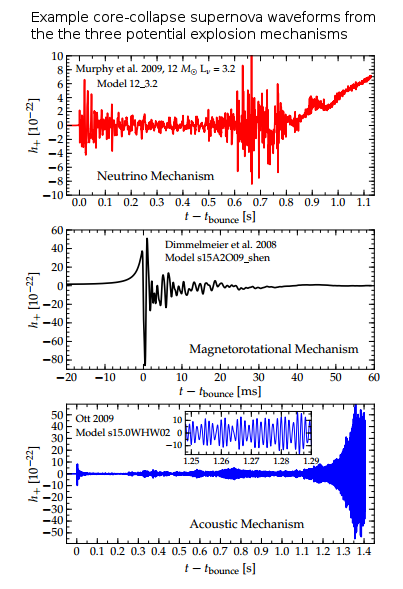
\includegraphics[scale=0.6]
	{figures/SN_waveforms.png}}
	\caption{\label{fig:model_waveforms} Examples of supernovae waveforms corresponding to the three frontrunner mechanisms for core-collapse supernovae explosion. Taken from \cite{Louge}.}
\end{figure}

%Current gravitational signal waveform catalogs for all three models are widely available. Additionally, generic waveform models for each of the three potential \sn{} mechanisms have been produced in \cite{Louge} using Principal Component Analysis and are available for comparison to \sn{} waveforms, as discussed in \ref{subsec:Classification}. 

It's also worth noting that galactic core-collapse SNe are rare events, occurring at a maximum likely rate of only a few per century. Advanced LIGO may be able to see most core-collapse SNe throughout the local group of galaxies (up to a distance of approximately 1 Mpc) \cite{Ott-SN_GWs}. 

%
%%
\section{Extracting the explosion mechanism from LIGO GW data} \label{MechExtract}

%
%%
\section{The importance of waveform reconstruction} 
